\newpage \clearpage
\section{Problem \#4}
\label{sec:prob4}

\subsection{Task}
Construct the minimum variance portfolio and tangent portfolio using 15 best performing stocks in US at the present day (use Yahoo! Finance: Market Data -> Market Stats -> Market Movers -> \% Gainers). Assume that short-selling is allowed. For the historical data consider the horizon of the last 2 years. Estimate the tail exponent for the returns of this portfolio. Compare with the tail exponent of the S\&P 500 index considered at the same horizon of 2 years.

\subsection{Problem description}

\paragraph*{Minimum-variance portfolio} --- the portfolio of risky assets with lowest variance ~\cite{Sel1}.

A portfolio of individually risky assets that, when taken together, result in the lowest possible risk level for the rate of expected return. Such a portfolio hedges each investment with an offsetting investment; the individual investor's choice on how much to offset investments depends on the level of risk and expected return he/she is willing to accept. The investments in a minimum variance portfolio are individually riskier than the portfolio as a whole. The name of the term comes from how it is mathematically expressed in Markowitz Portfolio Theory, in which volatility is used as a replacement for risk, and in which less variance in volatility correlates to less risk in an investment ~\cite{Sel2}.

\paragraph*{Modern Portfolio Theory} --- a theory of investing stating that every rational investor, at a given level of risk, will accept only the largest expected return. More specifically, modern portfolio theory attempts to account for risk and expected return mathematically to help the investor find a portfolio with the maximum return for the minimum about of risk. A Markowitz efficient portfolio represents just that: the most expected return at a given amount of risk (sometimes excluding zero risk). Harry Markowitz first began developing this theory in an article published in 1952 and received the Nobel prize for economics for his work in 1990 ~\cite{Sel3}.

\paragraph*{Tangent Portfolios} --- are portfolios of stocks and bonds designed for long-term investors. Since people hate losing money about twice as much as they enjoy making it, the Tangent Portfolios start by asking how much you would be prepared to lose in a worst-case scenario without bailing out of the market: 20\%, 25\%,or 33\%? Once the maximum loss level is selected, the Tangent Portfolios attempt to deliver a high rate of return for that amount of risk.
    Most investors tend to take on too much risk during good times ("buy high"), and then sell out during bad times ("sell low"), ruining their returns in the process. The Tangent Portfolios are designed to let you do well enough during both good times and bad to keep you in the markets throughout. This lets you reap the long-term benefits form investing in stocks and bonds with a simple, low-maintenance solution ~\cite{Sel4}.

\begin{figure}[b!]
	\centering
	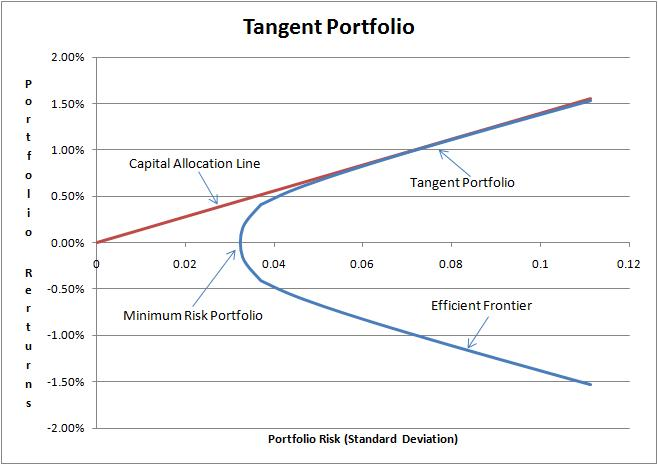
\includegraphics[width=1.0\textwidth,clip,keepaspectratio]{src/Pr4/1.jpg}
	\caption{Tangent portfolio defenition}
	\label{fig:s1}
\end{figure}
 
\paragraph*{S\&P 500} or the Standard \& Poor's 500, is a stock market index based on the market capitalizations of 500 large companies having common stock listed on the NYSE or NASDAQ. The S\&P 500 index components and their weightings are determined by S\&P Dow Jones Indices. It differs from other U.S. stock market indices, such as the Dow Jones Industrial Average or the Nasdaq Composite index, because of its diverse constituency and weighting methodology. It is one of the most commonly followed equity indices, and many consider it one of the best representations of the U.S. stock market, and a bellwether for the U.S. economy.The National Bureau of Economic Research has classified common stocks as a leading indicator of business cycles.

    The S\&P 500 was developed and continues to be maintained by S\&P Dow Jones Indices, a joint venture majority-owned byMcGraw Hill Financial. S\&P Dow Jones Indices publishes many stock market indices, such as the Dow Jones Industrial Average, S\&P MidCap 400, the S\&P SmallCap 600, and the S\&P Composite 1500. It is a free-float capitalization-weighted index, and has many ticker symbols, such as: GSPC, INX,and \$SPX ~\cite{Sel5}.


\subsection{Solution}

\subsection{Results}






























